\documentclass[11pt,a4paper,]{article}
\usepackage{lmodern}

\usepackage{amssymb,amsmath}
\usepackage{ifxetex,ifluatex}
\usepackage{fixltx2e} % provides \textsubscript
\ifnum 0\ifxetex 1\fi\ifluatex 1\fi=0 % if pdftex
  \usepackage[T1]{fontenc}
  \usepackage[utf8]{inputenc}
\else % if luatex or xelatex
  \usepackage{unicode-math}
  \defaultfontfeatures{Ligatures=TeX,Scale=MatchLowercase}
\fi
% use upquote if available, for straight quotes in verbatim environments
\IfFileExists{upquote.sty}{\usepackage{upquote}}{}
% use microtype if available
\IfFileExists{microtype.sty}{%
\usepackage[]{microtype}
\UseMicrotypeSet[protrusion]{basicmath} % disable protrusion for tt fonts
}{}
\PassOptionsToPackage{hyphens}{url} % url is loaded by hyperref
\usepackage[unicode=true]{hyperref}
\hypersetup{
            pdftitle={ETC513 Assignment 3: Comparison of Energy and Pollution by Country},
            pdfborder={0 0 0},
            breaklinks=true}
\urlstyle{same}  % don't use monospace font for urls
\usepackage{geometry}
\geometry{a4paper, centering, text={16cm,24cm}}
\usepackage[style=authoryear-comp,]{biblatex}
\addbibresource{references.bib}
\usepackage{longtable,booktabs}
% Fix footnotes in tables (requires footnote package)
\IfFileExists{footnote.sty}{\usepackage{footnote}\makesavenoteenv{long table}}{}
\IfFileExists{parskip.sty}{%
\usepackage{parskip}
}{% else
\setlength{\parindent}{0pt}
\setlength{\parskip}{6pt plus 2pt minus 1pt}
}
\setlength{\emergencystretch}{3em}  % prevent overfull lines
\providecommand{\tightlist}{%
  \setlength{\itemsep}{0pt}\setlength{\parskip}{0pt}}
\setcounter{secnumdepth}{5}

% set default figure placement to htbp
\makeatletter
\def\fps@figure{htbp}
\makeatother


\title{ETC513 Assignment 3: Comparison of Energy and Pollution by Country}

%% MONASH STUFF

%% CAPTIONS
\RequirePackage{caption}
\DeclareCaptionStyle{italic}[justification=centering]
 {labelfont={bf},textfont={it},labelsep=colon}
\captionsetup[figure]{style=italic,format=hang,singlelinecheck=true}
\captionsetup[table]{style=italic,format=hang,singlelinecheck=true}


%% FONT
\RequirePackage{bera}
\RequirePackage[charter,expert,sfscaled]{mathdesign}
\RequirePackage{fontawesome}

%% HEADERS AND FOOTERS
\RequirePackage{fancyhdr}
\pagestyle{fancy}
\rfoot{\Large\sffamily\raisebox{-0.1cm}{\textbf{\thepage}}}
\makeatletter
\lhead{\textsf{\expandafter{\@title}}}
\makeatother
\rhead{}
\cfoot{}
\setlength{\headheight}{15pt}
\renewcommand{\headrulewidth}{0.4pt}
\renewcommand{\footrulewidth}{0.4pt}
\fancypagestyle{plain}{%
\fancyhf{} % clear all header and footer fields
\fancyfoot[C]{\sffamily\thepage} % except the center
\renewcommand{\headrulewidth}{0pt}
\renewcommand{\footrulewidth}{0pt}}

%% MATHS
\RequirePackage{bm,amsmath}
\allowdisplaybreaks

%% GRAPHICS
\RequirePackage{graphicx}
\setcounter{topnumber}{2}
\setcounter{bottomnumber}{2}
\setcounter{totalnumber}{4}
\renewcommand{\topfraction}{0.85}
\renewcommand{\bottomfraction}{0.85}
\renewcommand{\textfraction}{0.15}
\renewcommand{\floatpagefraction}{0.8}


%\RequirePackage[section]{placeins}

%% SECTION TITLES


%% SECTION TITLES (NEW: Changing sections and subsections color)
\RequirePackage[compact,sf,bf]{titlesec}
\titleformat*{\section}{\Large\sf\bfseries\color[rgb]{0.8, 0.7, 0.1 }}
\titleformat*{\subsection}{\large\sf\bfseries\color[rgb]{0.8, 0.7, 0.1 }}
\titleformat*{\subsubsection}{\sf\bfseries\color[rgb]{0.8, 0.7, 0.1 }}
\titlespacing{\section}{0pt}{2ex}{.5ex}
\titlespacing{\subsection}{0pt}{1.5ex}{0ex}
\titlespacing{\subsubsection}{0pt}{.5ex}{0ex}


%% TITLE PAGE
\def\Date{\number\day}
\def\Month{\ifcase\month\or
 January\or February\or March\or April\or May\or June\or
 July\or August\or September\or October\or November\or December\fi}
\def\Year{\number\year}

%% LINE AND PAGE BREAKING
\sloppy
\clubpenalty = 10000
\widowpenalty = 10000
\brokenpenalty = 10000
\RequirePackage{microtype}

%% PARAGRAPH BREAKS
\setlength{\parskip}{1.4ex}
\setlength{\parindent}{0em}

%% HYPERLINKS
\RequirePackage{xcolor} % Needed for links
\definecolor{darkblue}{rgb}{0,0,.6}
\RequirePackage{url}

\makeatletter
\@ifpackageloaded{hyperref}{}{\RequirePackage{hyperref}}
\makeatother
\hypersetup{
     citecolor=0 0 0,
     breaklinks=true,
     bookmarksopen=true,
     bookmarksnumbered=true,
     linkcolor=darkblue,
     urlcolor=blue,
     citecolor=darkblue,
     colorlinks=true}

\usepackage[showonlyrefs]{mathtools}
\usepackage[no-weekday]{eukdate}

%% BIBLIOGRAPHY

\makeatletter
\@ifpackageloaded{biblatex}{}{\usepackage[style=authoryear-comp, backend=biber, natbib=true]{biblatex}}
\makeatother
\ExecuteBibliographyOptions{bibencoding=utf8,minnames=1,maxnames=3, maxbibnames=99,dashed=false,terseinits=true,giveninits=true,uniquename=false,uniquelist=false,doi=false, isbn=false,url=true,sortcites=false}

\DeclareFieldFormat{url}{\texttt{\url{#1}}}
\DeclareFieldFormat[article]{pages}{#1}
\DeclareFieldFormat[inproceedings]{pages}{\lowercase{pp.}#1}
\DeclareFieldFormat[incollection]{pages}{\lowercase{pp.}#1}
\DeclareFieldFormat[article]{volume}{\mkbibbold{#1}}
\DeclareFieldFormat[article]{number}{\mkbibparens{#1}}
\DeclareFieldFormat[article]{title}{\MakeCapital{#1}}
\DeclareFieldFormat[article]{url}{}
%\DeclareFieldFormat[book]{url}{}
%\DeclareFieldFormat[inbook]{url}{}
%\DeclareFieldFormat[incollection]{url}{}
%\DeclareFieldFormat[inproceedings]{url}{}
\DeclareFieldFormat[inproceedings]{title}{#1}
\DeclareFieldFormat{shorthandwidth}{#1}
%\DeclareFieldFormat{extrayear}{}
% No dot before number of articles
\usepackage{xpatch}
\xpatchbibmacro{volume+number+eid}{\setunit*{\adddot}}{}{}{}
% Remove In: for an article.
\renewbibmacro{in:}{%
  \ifentrytype{article}{}{%
  \printtext{\bibstring{in}\intitlepunct}}}

\AtEveryBibitem{\clearfield{month}}
\AtEveryCitekey{\clearfield{month}}

\makeatletter
\DeclareDelimFormat[cbx@textcite]{nameyeardelim}{\addspace}
\makeatother

\author{\sf\Large\textbf{ Shaohu Chen}\\ {\sf\large Master of Business Analytics(In Progress)\\[0.5cm]} \sf\Large\textbf{ Qian Duan}\\ {\sf\large Master of Business Analytics(In Progress)\\[0.5cm]} \sf\Large\textbf{ Tina Tsou}\\ {\sf\large Master of Business Analytics(In Progress)\\[0.5cm]}}

\date{\sf\Date~\Month~\Year}
\makeatletter
\lfoot{\sf Chen, Duan, Tsou: \@date}
\makeatother


%%%% PAGE STYLE FOR FRONT PAGE OF REPORTS

\makeatletter
\def\organization#1{\gdef\@organization{#1}}
\def\telephone#1{\gdef\@telephone{#1}}
\def\email#1{\gdef\@email{#1}}
\makeatother
  \organization{Australian Government COVID19}

  \def\name{Our consultancy \newline add names \&\newline add names}

  \telephone{(03) 9905 2478}

  \email{questions@company.com}                 %NEW: New email addresss

\def\webaddress{\url{http://company.com/stats/consulting/}} %NEW: URl
\def\abn{12 377 614 630}                                    % NEW: ABN
\def\logo{\includegraphics[width=6cm]{logo}}  %NEW: Changing logo
\def\extraspace{\vspace*{1.6cm}}
\makeatletter
\def\contactdetails{\faicon{phone} & \@telephone \\
                    \faicon{envelope} & \@email}
\makeatother

%%%% FRONT PAGE OF REPORTS

\def\reporttype{Report for}

\long\def\front#1#2#3{
\newpage
\begin{singlespacing}
\thispagestyle{empty}
\vspace*{-1.4cm}
\hspace*{-1.4cm}
\hbox to 16cm{
  \hbox to 6.5cm{\vbox to 14cm{\vbox to 25cm{
    \logo
    \vfill
    \parbox{6.3cm}{\raggedright
      \sf\color[rgb]{0.8, 0.7, 0.1 }    % NEW color 
      {\large\textbf{\name}}\par
      \vspace{.7cm}
      \tabcolsep=0.12cm\sf\small
      \begin{tabular}{@{}ll@{}}\contactdetails
      \end{tabular}
      \vspace*{0.3cm}\par
      ABN: \abn\par
    }
  }\vss}\hss}
  \hspace*{0.2cm}
  \hbox to 1cm{\vbox to 14cm{\rule{4pt}{26.8cm}\vss}\hss\hfill}  %NEW: Thicker line
  \hbox to 10cm{\vbox to 14cm{\vbox to 25cm{   
      \vspace*{3cm}\sf\raggedright
      \parbox{11cm}{\sf\raggedright\baselineskip=1.2cm
         \fontsize{24.88}{30}\color[rgb]{0, 0.29, 0.55}\sf\textbf{#1}}   % NEW: title color blue
      \par
      \vfill
      \large
      \vbox{\parskip=0.8cm #2}\par
      \vspace*{2cm}\par
      \reporttype\\[0.3cm]
      \hbox{#3}%\\[2cm]\
      \vspace*{1cm}
      {\large\sf\textbf{\Date~\Month~\Year}}
   }\vss}
  }}
\end{singlespacing}
\newpage
}

\makeatletter
\def\titlepage{\front{\expandafter{\@title}}{\@author}{\@organization}}
\makeatother

\usepackage{setspace}
\setstretch{1.5}

%% Any special functions or other packages can be loaded here.
\usepackage{dcolumn} 


\begin{document}
\titlepage

\section*{Introduction}

\section*{Step 1}

\section*{Step 2}

\section*{Step 3}

In the following section, we will be analyzing the relationship between \emph{Booking Type} and \emph{Exam Result}.

\begin{figure}

{\centering 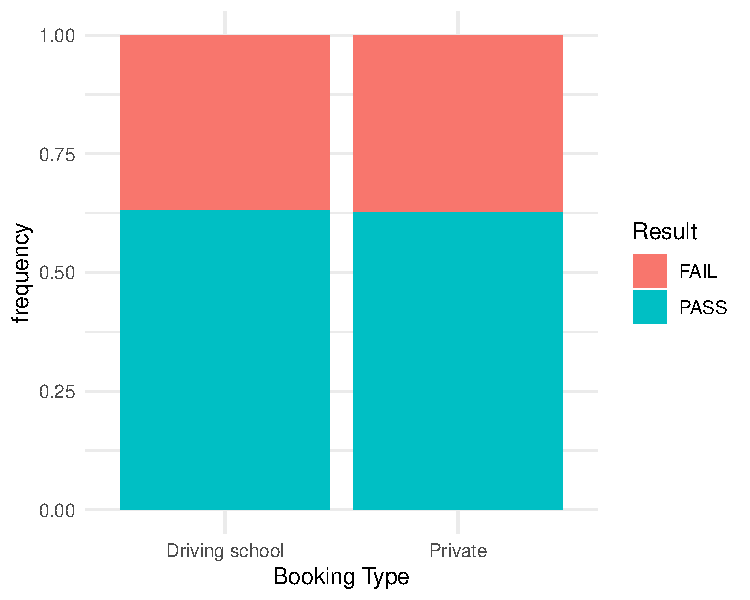
\includegraphics{Assignment4_files/figure-latex/frequency-1} 

}

\caption{Frequency Plot between Booking Type and Exam Result}\label{fig:frequency}
\end{figure}

The frequency plot, Figure \ref{fig:frequency}, between \emph{Booking Type} and \emph{Exam Result} shows that the percentages of people who passed the exam are similar for both driving school and private.

Since the response variable and predictor variable are categorical variables, they will have to be converted into dummy variables(0 \& 1). Then, following \textcite{logisticregregression}, I ran a logistic regression to analyze their relationship. The following is the formula for the regression \emph{logmodel}:

\(Y\)\textasciitilde{}\(B(p)\), \(log(\frac{p}{1-p}) = \beta_0 +\beta_1 X + \epsilon\)

\begin{itemize}
\item
  \(\beta_0\) is the intercept.
\item
  \(\beta_1\) is the coefficient of \emph{Booking Type\_Private}
\item
  X is \emph{Booking Type\_Private} taking values 0 or 1
\end{itemize}

\textbackslash begin\{table\}{[}!htbp{]} \centering 
\textbackslash caption\{Regression with \emph{Booking Type\_Private}\}
\label{}

\begin{tabular}{@{\extracolsep{5pt}}lD{.}{.}{-3} } 
\\[-1.8ex]\hline 
\hline \\[-1.8ex] 
 & \multicolumn{1}{c}{\textit{Dependent variable:}} \\ 
\cline{2-2} 
\\[-1.8ex] & \multicolumn{1}{c}{`Exam Result\_PASS`} \\ 
\hline \\[-1.8ex] 
 `Booking Type\_Private` & -0.061^{***} \\ 
  & (0.008) \\ 
  Constant & 0.559^{***} \\ 
  & (0.006) \\ 
 \hline \\[-1.8ex] 
Observations & \multicolumn{1}{c}{252,813} \\ 
Log Likelihood & \multicolumn{1}{c}{-166,739.600} \\ 
Akaike Inf. Crit. & \multicolumn{1}{c}{333,483.300} \\ 
\hline 
\hline \\[-1.8ex] 
\textit{Note:}  & \multicolumn{1}{r}{$^{*}$p$<$0.1; $^{**}$p$<$0.05; $^{***}$p$<$0.01} \\ 
\end{tabular}

\textbackslash end\{table\}

Table \ref{tab:results1} shows the regression summary. \emph{Booking Type\_Private} has p-value close to 0 which means it is statistically significant. Due to the variable being a dummy variable relative to booking type driving school, the coefficient indicates that \emph{Booking Type\_Private} affects the passing of an exam negatively compared to \emph{Booking Type\_Driving School}. Private booking reduces the log odds by 0.061.

\begin{table}

\caption{\label{tab:anova}Anova for logmodel}
\centering
\begin{tabular}[t]{lrrrrr}
\toprule
  & Df & Deviance & Resid. Df & Resid. Dev & Pr(>Chi)\\
\midrule
NULL & NA & NA & 252812 & 333534.7 & NA\\
`Booking Type\_Private` & 1 & 55.47238 & 252811 & 333479.3 & 0\\
\bottomrule
\end{tabular}
\end{table}

ANOVA test, table \ref{tab:anova}, on the \emph{logmodel} analyzes the table of deviance which shows how well the x variable is doing in comparison to the null model. Here we can see that the drop in deviance is quite small despite having low p-value.

Next, we test the fit of the model by looking at the receiver operating characteristic (ROC) curve.

\begin{figure}

{\centering 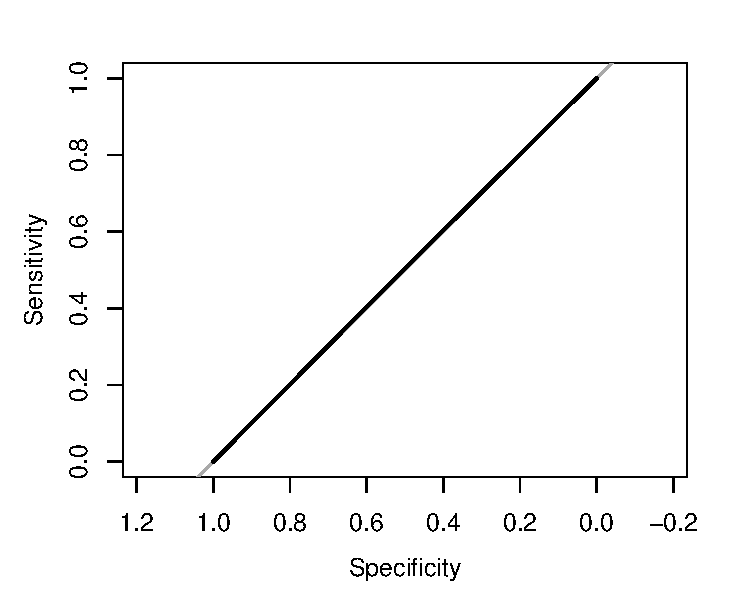
\includegraphics{Assignment4_files/figure-latex/roc-1} 

}

\caption{ROC Cuve of logmodel1}\label{fig:roc}
\end{figure}

Figure \ref{fig:roc} shows the ROC curve of the \emph{logmodel}. It is basically a 45 degree diagonal line which indicates the model has no discrimination ability.

Area under the curve ``\ldots gives the probability that the model correctly ranks such pairs of observations'' \textcite{bartlett_2014}. The area under the curve for this model is 0.5022363. In conclusion, the predictor just makes random guesses.

We try to improve the model by adding more variables to the function:

\(Y\)\textasciitilde{}\(B(p)\), \(log(\frac{p}{1-p}) = \beta_0 +\beta_1 X_1 +\beta_2 X_2 + \epsilon\)

\(X_2\) is \emph{Number of Examinations} taken by each examinee.

\begin{table}[!htbp] \centering 
  \caption{Regression Results} 
  \label{} 
\begin{tabular}{@{\extracolsep{5pt}}lD{.}{.}{-3} D{.}{.}{-3} } 
\\[-1.8ex]\hline 
\hline \\[-1.8ex] 
 & \multicolumn{2}{c}{\textit{Dependent variable:}} \\ 
\cline{2-3} 
\\[-1.8ex] & \multicolumn{2}{c}{`Exam Result\_PASS`} \\ 
\\[-1.8ex] & \multicolumn{1}{c}{(1)} & \multicolumn{1}{c}{(2)}\\ 
\hline \\[-1.8ex] 
 `Booking Type\_Private` & -0.061^{***} & -0.060^{***} \\ 
  & (0.008) & (0.008) \\ 
  `Number of Examinations` &  & 0.003^{***} \\ 
  &  & (0.0003) \\ 
  Constant & 0.559^{***} & 0.542^{***} \\ 
  & (0.006) & (0.006) \\ 
 \hline \\[-1.8ex] 
Observations & \multicolumn{1}{c}{252,813} & \multicolumn{1}{c}{252,813} \\ 
Log Likelihood & \multicolumn{1}{c}{-166,739.600} & \multicolumn{1}{c}{-166,699.100} \\ 
Akaike Inf. Crit. & \multicolumn{1}{c}{333,483.300} & \multicolumn{1}{c}{333,404.200} \\ 
\hline 
\hline \\[-1.8ex] 
\textit{Note:}  & \multicolumn{2}{r}{$^{*}$p$<$0.1; $^{**}$p$<$0.05; $^{***}$p$<$0.01} \\ 
\end{tabular} 
\end{table}

Table \ref{tab:comparison} shows the two regression summary side-by-side. The regression with \emph{Number of Examinations} has AIC of 333404. It is slightly lower than the AIC of the previous regression which was 333483. Thus, in comparison, having this one extra variable improved the function significantly (statistically). However, a simple calculation of area under ROC curve for logmodel2 indicates that the model is even worse than the first.

\begin{verbatim}
## Area under the curve: 0.486
\end{verbatim}

\section*{Conclusion}

In conclusion, we've shown that higher pass rate in certain districts is not always an absolute reflection on whether the district has better driving program. Rather, it is an outcome of locations with lower examinees in general. For locations with more examinees, there would be more variations in their outcome thus more fails.

Next, we shown that automatic cars have the lowest pass rate overall, and that motorcycle (over 250cc) has the highest pass rate. Older people (66 and above) also tend to fail their vehicle tests more. But ultimately pass rate for each vehicle type and majority of the age group is over 50\%.

Last but not least, although, there is statistical relationship between the booking type and the exam outcome, the affect is pretty small. Furthermore, the current variables are inadequate in creating a good model to predict the outcome.

This is also a shortcoming with the data we currently have. Because it contains very limited variables, it is hard to create a better fit model that can predict the outcome accurately.

\printbibliography

\end{document}
